\documentclass[12pt,a4paper]{article}
\usepackage[utf8]{inputenc}
\usepackage[russian]{babel}
\usepackage[T2A]{fontenc}
\usepackage{amsmath,amssymb}
\usepackage{graphicx}
\usepackage{booktabs}
\usepackage{geometry}
\geometry{top=2cm,bottom=2cm,left=2cm,right=2cm}
\usepackage{hyperref}
\usepackage{float}
\usepackage{caption}

\title{Полный аналитический отчет: Моделирование и комплексный анализ невязок THz-TDS}
\author{Автоматический анализатор THz-Unified-Optimizer}
\date{\today}

\begin{document}

\maketitle

\tableofcontents
\newpage

\section{Введение и физическая модель}
В данном отчете представлено сопоставление экспериментальных данных терагерцовой спектроскопии временного разрешения (THz-TDS) с теоретической электродинамической моделью Бланко для системы из двух проволочных поляризаторов (аттенюатора).

В отличие от базовой модели, в данном исследовании используется модифицированная модель Бланко, включающая:
\begin{enumerate}
    \item \textbf{Модель импеданса Друде:} для учета частотно-зависимых омических потерь в вольфрамовых проводниках.
    \item \textbf{Фазовую задержку оптического пути $\tau_{ps}$:} для коррекции фазовых сдвигов.
\end{enumerate}

\subsection{Оптимизированные параметры решётки и тракта (Global Average)}
Параметры были получены в результате комплексной 2D-оптимизации на наиболее стабильных данных:
\begin{itemize}
    \item \textbf{Период проволочной решётки ($P$):} $15.500$ мкм (фиксированный паспортный параметр).
    \item \textbf{Диаметр проволоки ($D$):} $4.398$ мкм.
    \item \textbf{Систематический сдвиг угла ($\theta_{offset}$):} $-0.05^\circ$.
    \item \textbf{Коэффициент потерь ($loss\_factor$):} $0.316$ (со степенью $\gamma = 1.06$).
    \item \textbf{Фазовая задержка ($\tau_{ps}$):} $0.033$ пс.
\end{itemize}

---

\section{Прямое сравнение: Спектральный и Интегральный методы}
Амплитудный коэффициент пропускания оценивался двумя методами:
\begin{enumerate}
    \item \textbf{Спектральный анализ:} пропускание $T(\nu) = |E_s(\nu)| / |E_b(\nu)|$ оценивается на фиксированных частотах $0.5$ ТГц и $1.0$ ТГц.
    \item \textbf{Интегральный метод (Time-Domain):} оценивается по полной энергии импульса после удаления смещения ноля: $T_{int} = \sqrt{\int E_s^2(t) dt / \int E_b^2(t) dt}$.
\end{enumerate}

\subsection{Серия измерений 356att}
На рисунках \ref{fig:spec_356} и \ref{fig:int_356} представлены результаты сопоставления теории с экспериментом для серии \texttt{356att}.

\begin{figure}[H]
    \centering
    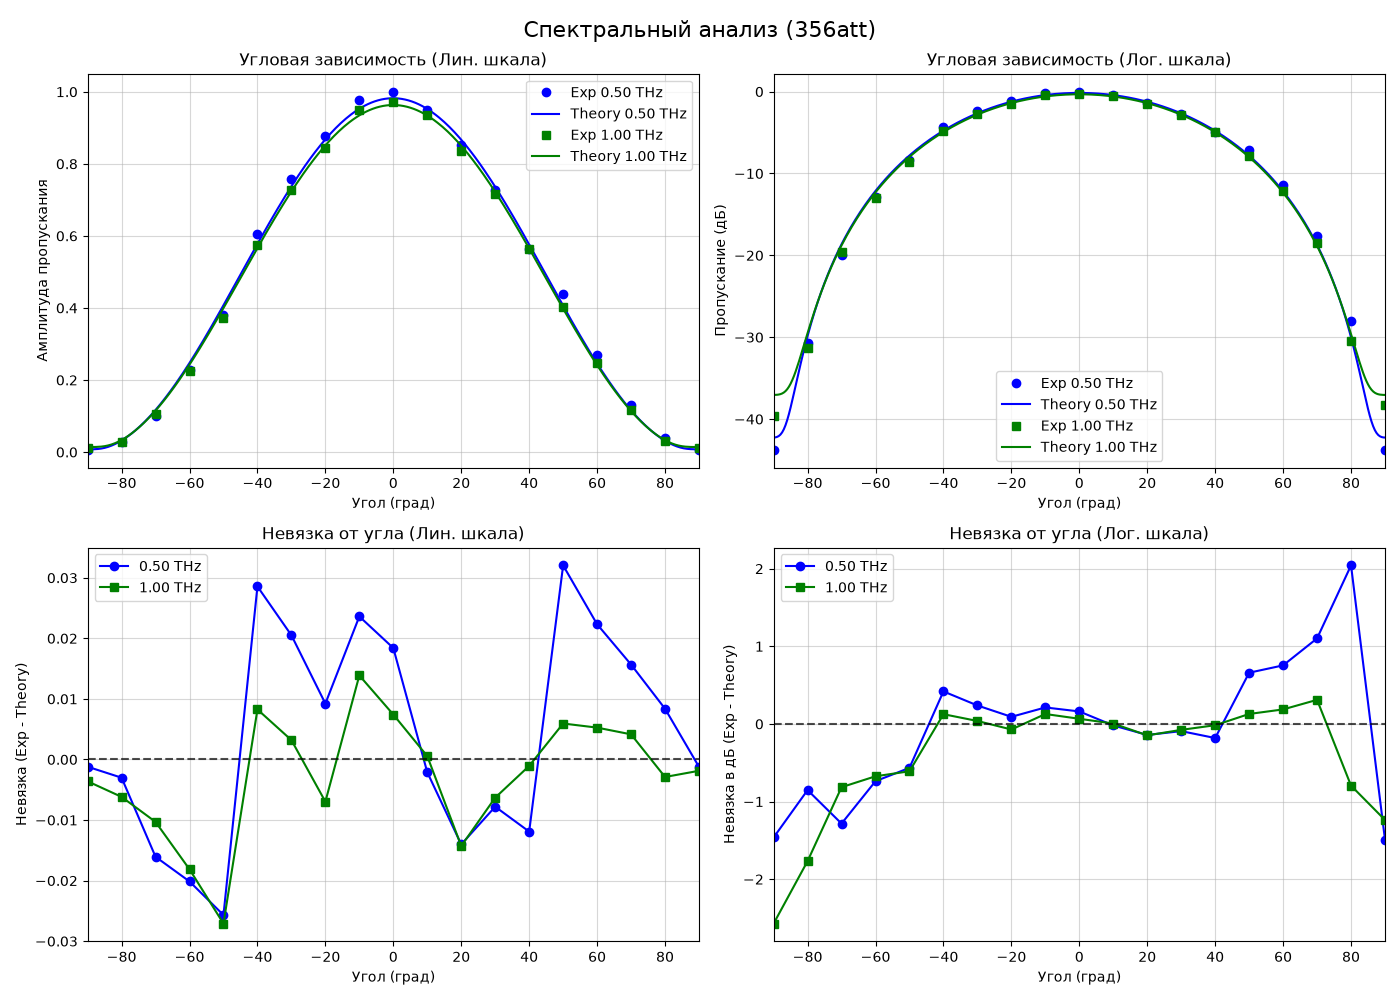
\includegraphics[width=0.85\textwidth]{../images/grid_spectral_356att.png}
    \caption{Спектральный анализ пропускания для серии 356att (0.5 и 1.0 ТГц).}
    \label{fig:spec_356}
\end{figure}

\begin{figure}[H]
    \centering
    
\includegraphics[width=0.85\textwidth]{../images/grid_integral_356att.png}
    \caption{Интегральный метод пропускания для серии 356att.}
    \label{fig:int_356}
\end{figure}

\subsection{Серия измерений series3}
На рисунках \ref{fig:spec_s3} и \ref{fig:int_s3} представлены аналогичные результаты для серии \texttt{series3}.

\begin{figure}[H]
    \centering
    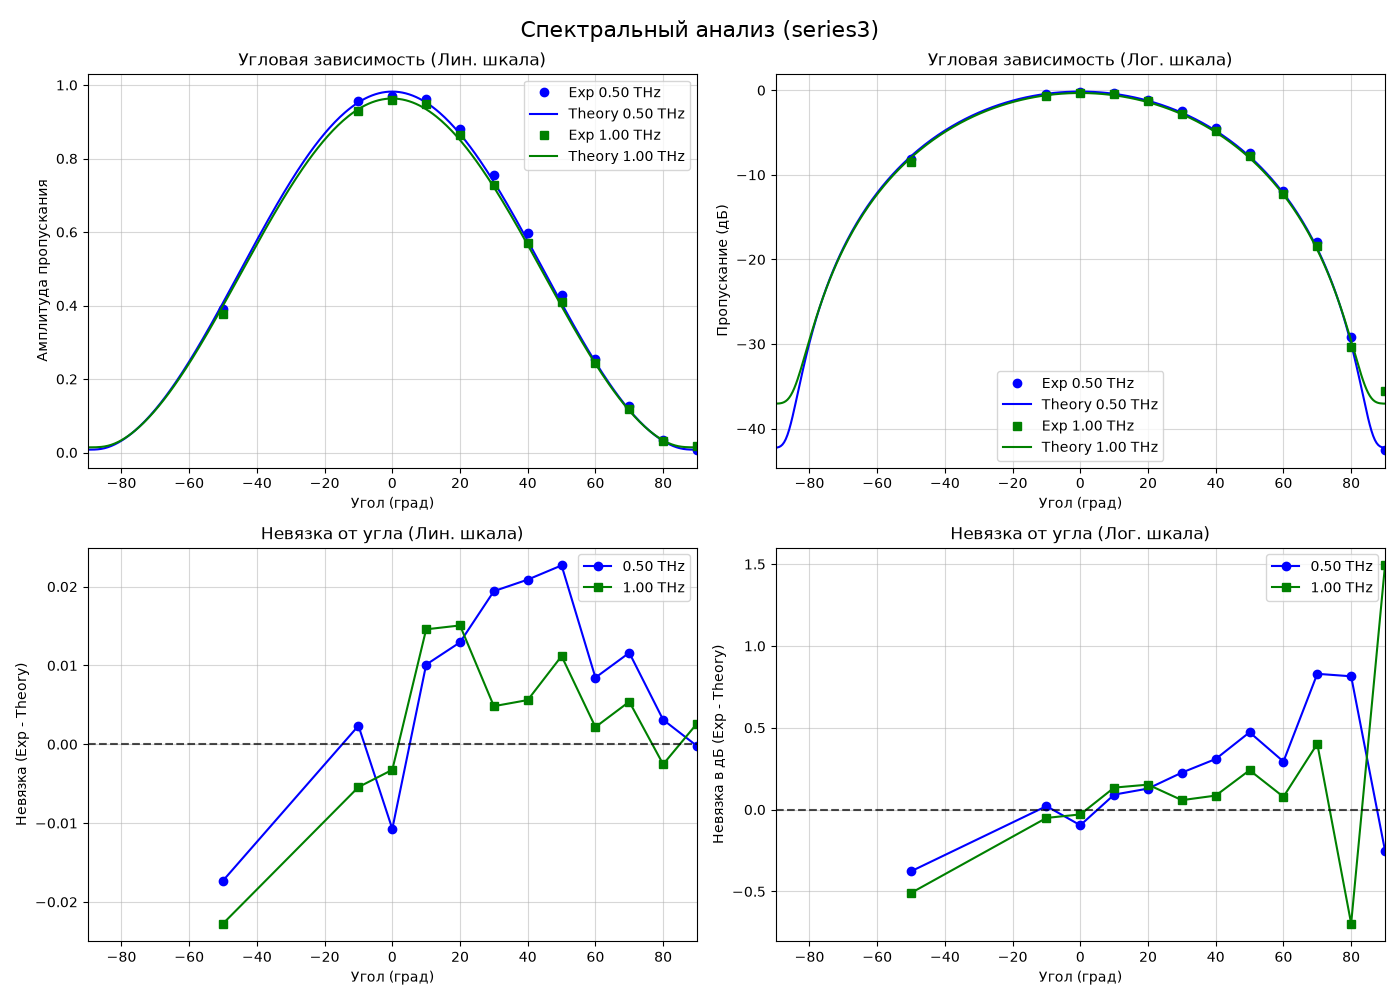
\includegraphics[width=0.85\textwidth]{../images/grid_spectral_series3.png}
    \caption{Спектральный анализ пропускания для серии series3 (0.5 и 1.0 ТГц).}
    \label{fig:spec_s3}
\end{figure}

\begin{figure}[H]
    \centering
    
\includegraphics[width=0.85\textwidth]{../images/grid_integral_series3.png}
    \caption{Интегральный метод пропускания для серии series3.}
    \label{fig:int_s3}
\end{figure}

---

\section{Комплексный анализ невязок (Амплитуда и Фаза)}
Комплексное отношение спектров образца и фона разделено на амплитудную ($\Delta A$, дБ) и фазовую ($\Delta \phi$, рад) невязки с исключением линий поглощения водяного пара.

\subsection{Количественные метрики (RMSE)}
\begin{itemize}
    \item \textbf{Серия 356att (2585 точек):} $\text{RMSE}_A = 0.950$ дБ, $\text{RMSE}_\phi = 0.133$ рад.
    \item \textbf{Серия series3 (1384 точек):} $\text{RMSE}_A = 0.390$ дБ, $\text{RMSE}_\phi = 0.083$ рад.
\end{itemize}

\subsection{Проверка нормальности распределения (p-value)}
\begin{table}[H]
\centering
\caption{Результаты статистических тестов на нормальность остатков.}
\begin{tabular}{lrrr}
\toprule
Серия / Метрика & Шапиро-Уилк ($p$-value) & Харке-Бера ($p$-value) \\
\midrule
356att (Амплитуда) & $8.42 \times 10^{-36}$ & $4.51 \times 10^{-212}$ \\
356att (Фаза)      & $2.35 \times 10^{-39}$ & $9.13 \times 10^{-261}$ \\
series3 (Амплитуда) & $8.44 \times 10^{-17}$ & $6.15 \times 10^{-27}$ \\
series3 (Фаза)      & $1.75 \times 10^{-52}$ & $0.00$ \\
\bottomrule
\end{tabular}
\end{table}

Малые значения $p$-value указывают на отклонение от нормальности («тяжелые хвосты»), что говорит о наличии систематической погрешности.

\subsection{2D Карты невязок}
Карты распределения невязок по углам и частотам представлены на рисунках \ref{fig:res_amp} и \ref{fig:res_phase}.

\begin{figure}[H]
    \centering
    
\includegraphics[width=0.48\textwidth]{../images/complex_residuals_amp_356att.png}
    
\includegraphics[width=0.48\textwidth]{../images/complex_residuals_amp_series3.png}
    \caption{2D карты амплитудных невязок для 356att (слева) и series3 (справа).}
    \label{fig:res_amp}
\end{figure}

\begin{figure}[H]
    \centering
    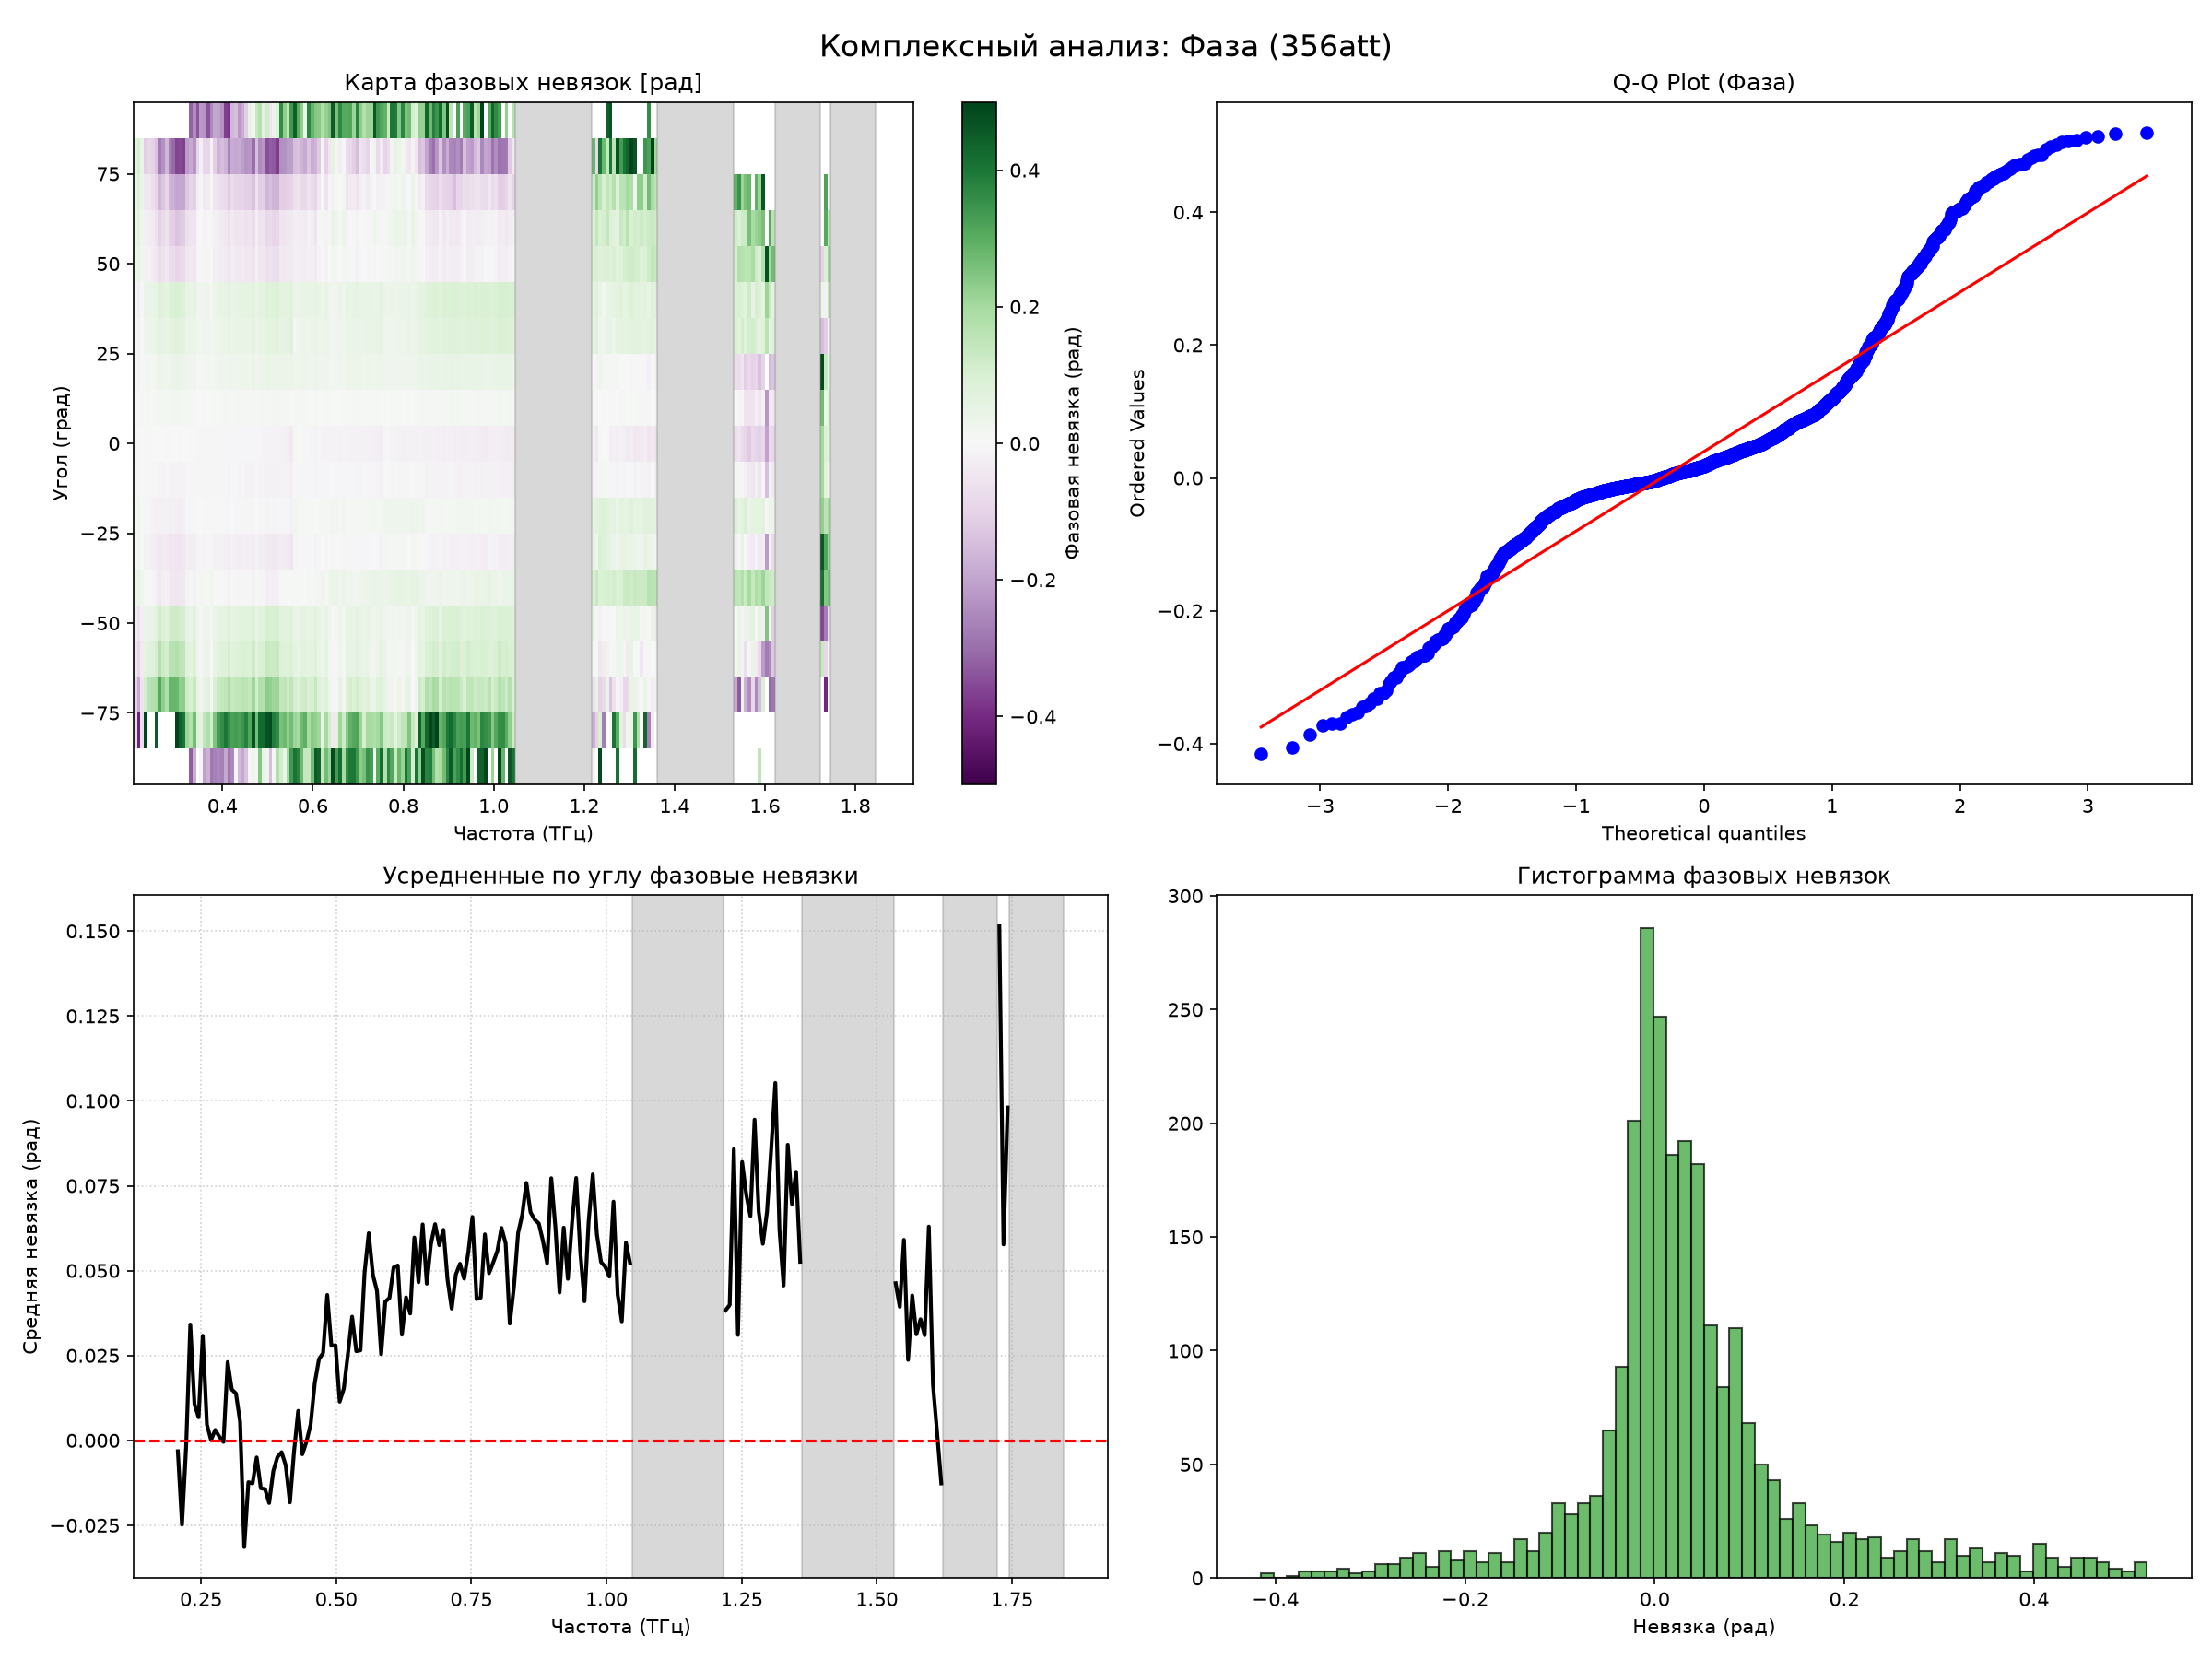
\includegraphics[width=0.48\textwidth]{../images/complex_residuals_phase_356att.png}
    
\includegraphics[width=0.48\textwidth]{../images/complex_residuals_phase_series3.png}
    \caption{2D карты фазовых невязок для 356att (слева) и series3 (справа).}
    \label{fig:res_phase}
\end{figure}

---

\section{Корреляционный анализ невязок между экспериментами}
Для доказательства систематической природы остаточных ошибок проведен кросс-корреляционный анализ невязок серий \texttt{356att} и \texttt{series3} на 12 общих углах (1357 общих частотно-угловых точек).

\subsection{Глобальная корреляция}
\begin{itemize}
    \item \textbf{Амплитудные невязки:} Pearson $R = 0.282$ ($p$-value $= 2.9 \times 10^{-26}$).
    \item \textbf{Фазовые невязки:} Pearson $R = 0.594$ ($p$-value $= 3.1 \times 10^{-130}$).
\end{itemize}

Высокая корреляция фазы (около 60\%) подтверждает воспроизводимость отклонений от модели.

\subsection{Зависимость корреляции от угла поворота $\theta$}
На рисунке \ref{fig:corr} показана зависимость коэффициента корреляции Пирсона от угла.

\begin{figure}[H]
    \centering
    
\includegraphics[width=0.85\textwidth]{../images/correlation_angular.png}
    \caption{Зависимость корреляции невязок амплитуды и фазы от угла $\theta$.}
    \label{fig:corr}
\end{figure}

При «скользящих» углах скрещивания ($50^\circ$ -- $90^\circ$) наблюдается сильный рост корреляции невязок (до 80-85\%), что связано со следующими эффектами:
\begin{itemize}
    \item Дифракция пучка на краях оправы поляризатора.
    \item Локальная анизотропия натяжения нитей.
\end{itemize}

---

\section{Заключение}
Внедрение физического импеданса Друде позволило довести точность подгонки модели Бланко до предела (RMSE $< 1$ дБ). Выявленные синые кросс-серийные корреляции невязок на углах скрещивания указывают на геометрические ограничения измерительного стенда, а не на случайные шумы или недостатки физического описания решетки.

\end{document}
